
\documentclass[10pt]{beamer}
\RequirePackage{pgfcore}
\usetheme{default}
\setbeamertemplate{blocks}[rounded][shadow=true]
\setbeamercovered{transparent}
\setbeamertemplate{navigation symbols}{}
\usefonttheme[stillsansseriflarge]{serif}
\newcommand{\E}{\mathbb{E}} 	%Expectation operator
\usepackage{parskip}
\usepackage{ textcomp }
\usepackage{lmodern}
\usepackage{color}
\usepackage{tabulary}
\usepackage{array, multirow}
\usepackage{colortbl}
\usepackage{animate}
\usepackage{graphicx, bm}
% \usepackage{algorithm,algorithmic}
\newcommand{\norm}[1]{\left\lVert#1\right\rVert}



\title{Frailty Classifier Project \\ Modeling Strategy}
\author{Andrew Crane-Droesch}
\date{\today}



\begin{document}

    \begin{frame}
    \titlepage
    \end{frame}


\begin{frame}{Outline}
\begin{enumerate}
\item Brief overview of the project
\item Annotation:  why/what/how
\item Word embeddings
\item Modeling
\item Active learning
\end{enumerate}
\end{frame}

\begin{frame}{Project overview}
``Classify potentially preventable phenotypes of hospital admission among community-dwelling patients with chronic lung diseases using NLP within EHR data''
\begin{itemize}
\item Many hospital admissions are ``low value''
	\begin{itemize}
	\item Perhaps they could have been prevented
	\item Patients often prefer not to be hospitalized
	\end{itemize}
\item It is not obvious \textit{a priori} which people would be candidates for preventative measures, or what preventative measures to take
\item This project builds on a related project that \textit{identifies phenotypes} of people who are at high risk of hospitalization (``frailty'')
\item The \textbf{immediate aim} is to identify \textit{actionable aspects} of frailty
\item Later, the goal is to use this to identify patients at high risk of being hospitalized, who have \textit{\textbf{actionable}} risk reduction avenues
	\begin{itemize}
	\item Pulmonary rehab might prevent some respiratory crises
	\item Physical therapy might enable pulmonary rehab
	\item Installing grab bars in bathrooms might prevent falls
	\end{itemize}
\end{itemize}
\end{frame}

\begin{frame}{Project workflow}
\begin{enumerate}
\item Download and process free text notes $\rightarrow$
\item Annotation of spans of notes that are {\color{red}\textbf{positive}} or {\color{green}\textbf{negative}} for the following actionable aspects of frailty:
	\begin{itemize}
	\item Fall risk
	\item Musculo-skeletal problems
	\item Respiratory impairment
	\item Nutrition problems
	\end{itemize}
\item Fitting models to predict the annotations from the spans
\item Using the fitted models to serve new batches of notes to annotate
\item Repeating 2, 3, and 4 until the models are good enough to classify text in the wild
\end{enumerate}
\end{frame}

\begin{frame}{Data munging and text processing}
\textbf{Population}:  all patients who've been at Penn for $>$1 year, with at least one of several diagnoses relating to chronic lung disease.
Pipeline:
\begin{itemize}
\item Pull all signed \textbf{outpatient} progress notes from patients with relevant diagnoses
\item Concatenate notes for individual patients into 6-month windows, simulating a prospective trial where targeting is done based on 6 months of history
\end{itemize}
\end{frame}

\begin{frame}{Summary stats}
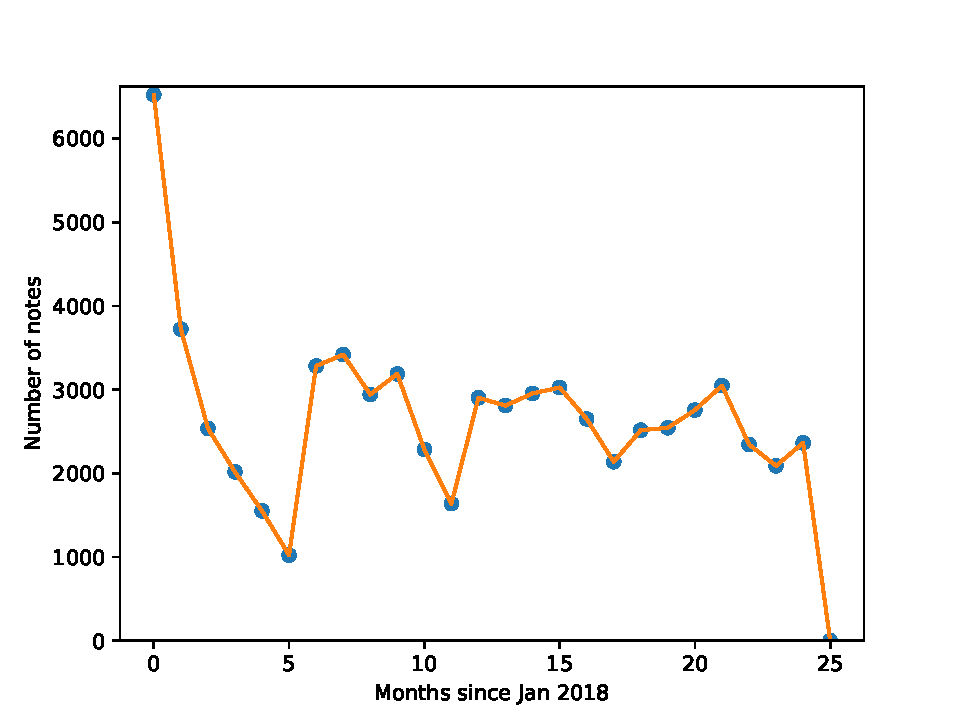
\includegraphics[width = .48\textwidth]{/Users/crandrew/projects/GW_PAIR_frailty_classifier/figures/pat_per_month.pdf}
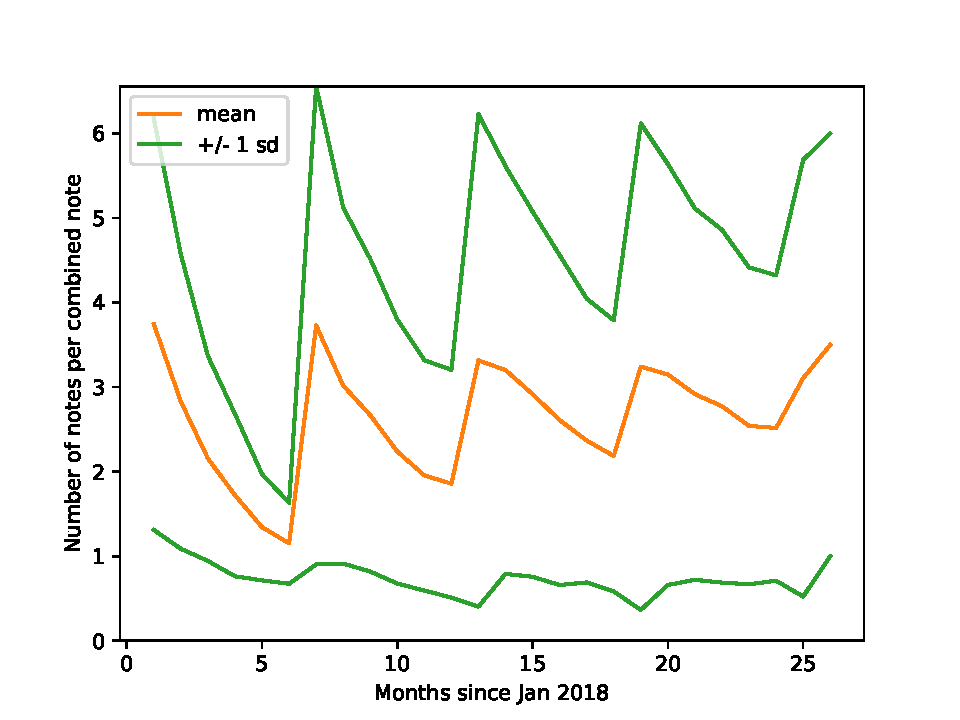
\includegraphics[width = .48\textwidth]{/Users/crandrew/projects/GW_PAIR_frailty_classifier/figures/n_notes.pdf}
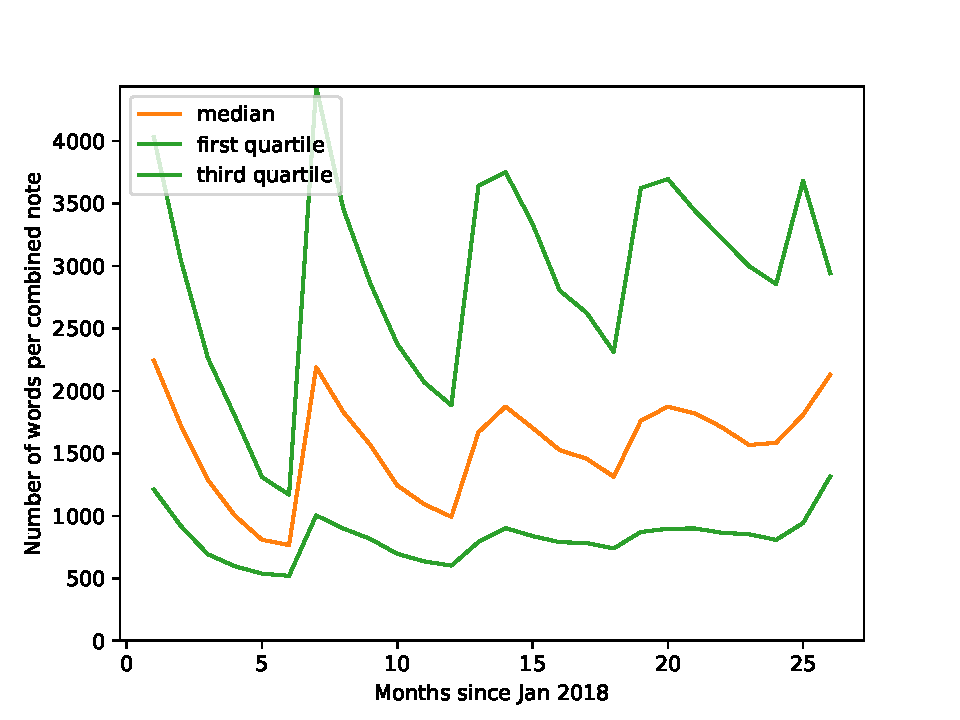
\includegraphics[width = .48\textwidth]{/Users/crandrew/projects/GW_PAIR_frailty_classifier/figures/n_words.pdf}
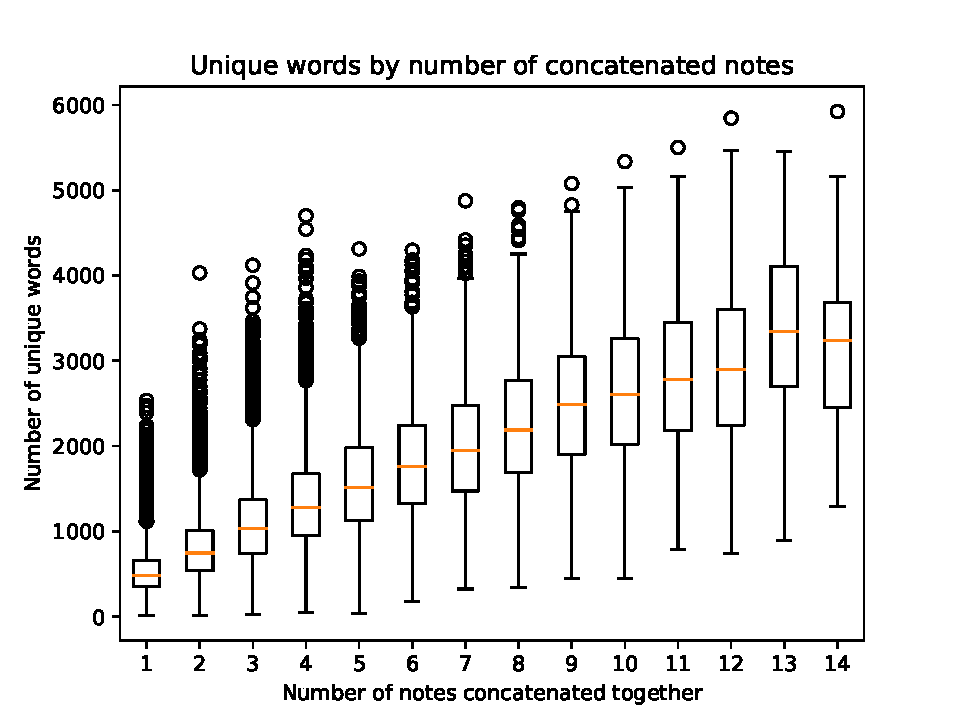
\includegraphics[width = .48\textwidth]{/Users/crandrew/projects/GW_PAIR_frailty_classifier/figures/nnotes_by_uwords.pdf}
\end{frame}

\begin{frame}{Annotation}
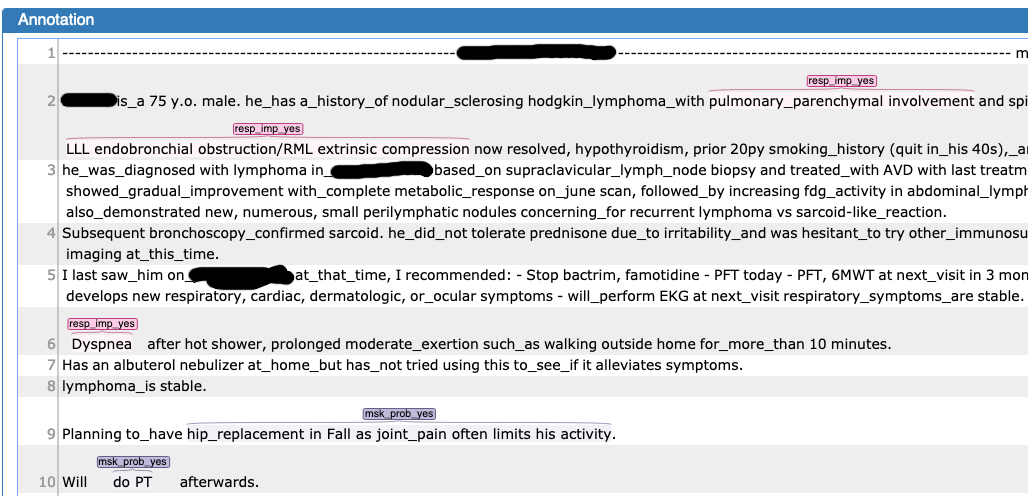
\includegraphics[width = 1.10\textwidth]{/Users/crandrew/projects/GW_PAIR_frailty_classifier/figures/webanno.png}
\end{frame}

\begin{frame}{Tokenization and label processing}
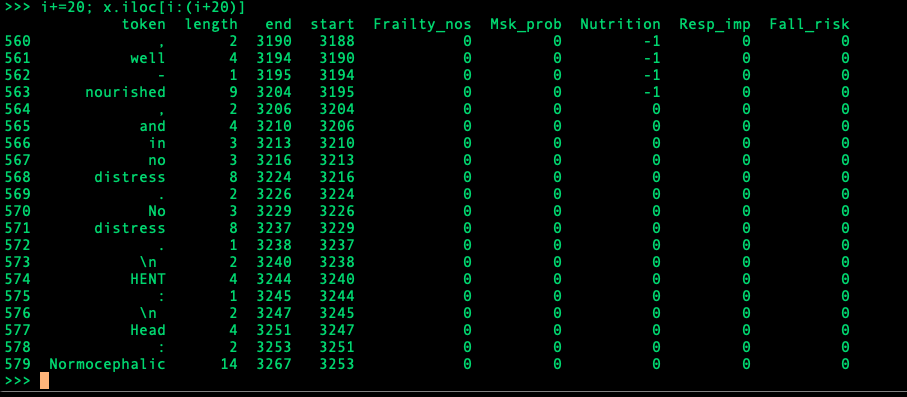
\includegraphics[width = 1\textwidth]{/Users/crandrew/projects/GW_PAIR_frailty_classifier/figures/df_slice.png}
$\uparrow$ this is the raw data.  How can we use the token to predict the label?
\end{frame}

\begin{frame}
\huge{Word embeddings}
\end{frame}


\begin{frame}{Document matrix}
Start with a sparse matrix ``one-hot'' encoded representation of a document:
\begin{itemize}
	\item The rows correspond to positions in a sequence
	\item The columns correspond to unique words
	\item The sum of the matrix equals the number of rows
\end{itemize}
\[  \bm{D} \equiv
\begin{array}{c|cccccc}
     & I & am & Sam & would & you & like \\
     \hline
I    & 1 & 0  & 0   & 0     & 0   &  0 \\
am   & 0 & 1  & 0   & 0     & 0   &  0 \\
Sam  & 0 & 0  & 1   & 0     & 0   &  0 \\
Sam  & 0 & 0  & 1   & 0     & 0   &  0 \\
I    & 1 & 0  & 0   & 0     & 0   &  0 \\
am   & 0 & 1  & 0   & 0     & 0   &  0 \\
would& 0 & 0  & 0   & 1     & 0   &  0 \\
you  & 0 & 0  & 0   & 0     & 1   &  0 \\
like & 0 & 0  & 0   & 0     & 0   &  1 \\
\end{array}\] 
Call it $\bm{D}$.  It has dimensions $N\times V$ -- total words by unique words.
\end{frame}


\begin{frame}{Document matrix}
\begin{itemize}
	\item Document matrices are \textit{sparse}.  Lots of zeros.  
	\item They are high-dimensional.  Using $\bm{D}$ directly as a design matrix in a model is generally inefficient.
	\item A document matrix doesn't explicitly encode any information about how words might be similar to each other.  Synonyms are wholly different from each other.
	\begin{itemize}
		\item The euclidean distance between any two word vectors (rows in the matrix) will always be $\sqrt{2}$
		\item The cosine similarity will always be zero
	\end{itemize}
	\item Summing them column-wise makes a unigram matrix:
	\[ 
\begin{array}{c|cccccc}
     & I & am & Sam & would & you & like \\
     \hline
1-gram    & 2 & 2  & 2   & 1     & 1   &  1 \\
\end{array}\] 
\end{itemize}
\end{frame}

\begin{frame}{Embeddings}
Embeddings attempt to do the following:
\begin{itemize}
\item Reduce the dimensionality of $\bm{D}$ without losing too much information
\item Capture the similarity between similar words
\end{itemize}
Different embedding methods do this in different ways, but all create analogous output:
\begin{itemize}
\item word2vec, fasttext, GloVe
\end{itemize}
\end{frame}

\begin{frame}{Embeddings in pictures}
\centering
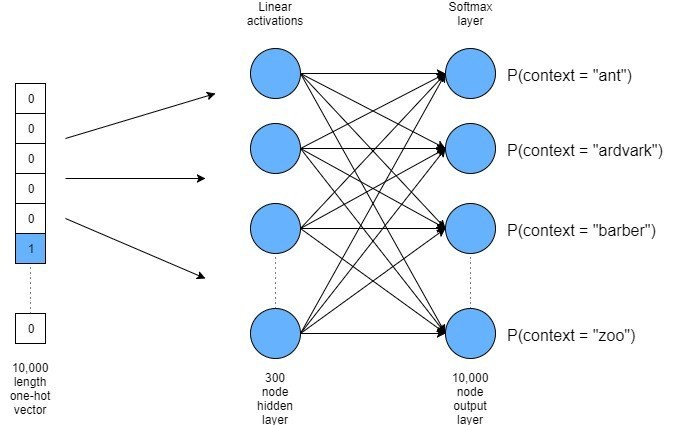
\includegraphics[width=.9\textwidth]{embeddings_example.jpeg}
\end{frame}

\begin{frame}{Embeddings in pictures}
\centering
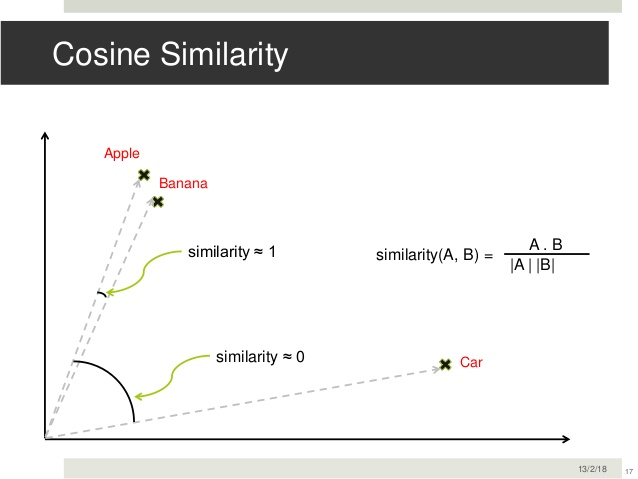
\includegraphics[width=.9\textwidth]{cosine_sim_2.jpg}
\end{frame}

\begin{frame}{Embeddings in math}
(a simple) Embedding model:
\[
\bm{D} = s\left(\bm{D\Gamma}_0\bm{\Gamma}_1\right) + \epsilon
\]
where:
\begin{itemize}
\item $\bm{D}$ is the document matrix, dimension $N\times V$
\item $\bm{\Gamma}_0$ is the first weight matrix.  It has dimension $V \times U$, where $U << V$.  It is responsible for ``embedding'' $\bm{D}$ in a lower-dimensional space
\item $\bm{\Gamma}_1$ is the second weight matrix.  Its dimension is $U \times V$.  It is responsible for taking the lower-dimensional representation and bringing it back to the original resolution.
\item $s()$ is the softmax function.  It maps the maps real numbers to a vector of probabilities summing to 1.
\item $\epsilon$ is the error to be minimized.  As the bottleneck gets skinnier (i.e.: as $U$ gets smaller), $\epsilon$ will have to increase.
\end{itemize}
\end{frame}

\begin{frame}{Embeddings in math}
(a simple) Embedding model:
\[
\bm{D} = s\left(\bm{D\Gamma}_0\bm{\Gamma}_1\right) + \epsilon
\]
where:
\begin{itemize}
\item The embedded text, call it $\bm{E}$, is defined as $\bm{D\Gamma_0}$ (dimension $N \times U$)
\item (most) Embedding models are trained by computing the derivatives of the parameter matrices $\bm{\Gamma}_0, \bm{\Gamma}_1$ with respect to a loss function, changing the parameters to make the loss smaller, and then recomputing the derivatives and repeating.  This is backpropagation.
\item the error $\epsilon$ is implicit.  The goal is to minimize it, to get the best possible $\bm{\Gamma}$.  But as the dimension of $\bm{\Gamma}$ gets smaller, this gets harder to do.
\end{itemize}
\end{frame}

\begin{frame}{Embeddings in practice}
Training and using embeddings are separate processes.  Trained embedding models give you $\bm{\Gamma}_0$.  You then supply your own text to multiply it against.  For example, take $\bm{D}$ to be our Dr Seuss example from before.  The embeddings $\bm\Gamma_0$ might look like this:
\[  \bm{\Gamma}_0 \equiv
\begin{array}{c|cccccc}
     & u1 & u2 \\
     \hline
I    & 1 & 2 \\
am   & 3 & 4  \\
Sam  & 5 & 6   \\
would& 7 & 8  \\
you  & 9 & 10  \\
like & 11 & 12  \\
\end{array}\] 
(Note that the entries of the matrix are totally unrealistic in this example)

\end{frame}

\begin{frame}{Embeddings in practice}
Say you wanted to embed the phrase ``I like Sam'' into this two-dimensional space:

\[ 
\left[
\begin{array}{c|cccccc}
I    & 1 & 0  & 0   & 0     & 0   &  0 \\
like & 0 & 0  & 0   & 0     & 0   &  1 \\
Sam  & 0 & 0  & 1   & 0     & 0   &  0 \\
\end{array}\right]
\left[\begin{array}{c|cccccc}
     & u1 & u2 \\
     \hline
I    & 1 & 2 \\
am   & 3 & 4  \\
Sam  & 5 & 6   \\
would& 7 & 8  \\
you  & 9 & 10  \\
like & 11 & 12  \\
\end{array}\right] = 
\left[
\begin{array}{c|cccccc}
     & u1 & u2 \\
     \hline
I    & 1 & 2 \\
like & 11 & 12  \\
Sam  & 5 & 6   \\
\end{array}
\right]
\] 
Because the the document matrix $\bm{D}$ has only one ``1'' per row, this matrix multiplication is the same as a ``lookup'' operation.

Still, the matrix notation will come in handy later.

\end{frame}


\begin{frame}{Word embeddings to sentence or span embeddings}
Supervised learning jobs can all be conceptualized as 
\[
y = f(\bm{X}) + \epsilon
\]
where $y$ is some label and $\bm{X}$ is a matrix of features.  So let's add a label to our toy example:


\[
\begin{array}{c|cccccc|c}
     & I & am & Sam & would & you & like & \text{\textbf{label}}\\
     \hline
I    & 1 & 0  & 0   & 0     & 0   &  0  & 0\\
am   & 0 & 1  & 0   & 0     & 0   &  0  & 0\\
Sam  & 0 & 0  & 1   & 0     & 0   &  0  & 1\\
Sam  & 0 & 0  & 1   & 0     & 0   &  0  & 0\\
I    & 1 & 0  & 0   & 0     & 0   &  0  & 0\\
am   & 0 & 1  & 0   & 0     & 0   &  0  & 0\\
would& 0 & 0  & 0   & 1     & 0   &  0  & 1\\
you  & 0 & 0  & 0   & 0     & 1   &  0  & 1\\
like & 0 & 0  & 0   & 0     & 0   &  1  & 0\\
\end{array}\] 
(I labeled words that come after a verb)
\end{frame}

\begin{frame}{Word embeddings to sentence or span embeddings}
If we fit 
\[
\text{\textbf{label}} = f(\bm{D}) + \epsilon
\]
or 
\[
\text{\textbf{label}} = f(\bm{E}) + \epsilon
\]
our model would do nothing but capture the correlations between individual words and labels.  But what if we want to capture the surrounding context?

First, let's remember that the matrix equation above is the same as 
\[
label_i = f(E_i) + \epsilon
\]
where $i$ indexes rows from 1 to $N$.  A natural strategy could be to include lags and leads:
\[
label_i = f(E_i, E_{i-1}, E_{i+1}) + \epsilon
\]
But lots of other possibilities exist.
\end{frame}


\begin{frame}{Word embeddings to sentence or span embeddings}
Consider the span ``I am Sam''.  Its embedding is:
\[\left[\begin{array}{c|cc|c}
     & u1 & u2 & \text{\textbf{label}}\\
     \hline
I    & 1 & 2 & 0\\
am   & 3 & 4 & 0 \\
Sam  & 5 & 6 & 1  \\
\end{array}\right]\]
The centroid word is ``am'', which is associated with a label of zero.  How do we associate information about the surrounding words with that zero label?  Several options, all of which involve ``windowing'':
\begin{itemize}
\item Lags and leads
\item span-wise maxes and mins, averages
\end{itemize}
\[\left[\begin{array}{c|cc|c|cc|cc|cc|cc}
     & u1 & u2 & \text{\textbf{label}} & \multicolumn{2}{c|}{lag}& \multicolumn{2}{c|}{lead} & \multicolumn{2}{c}{min}& \multicolumn{2}{c|}{max}\\
     \hline
am   & 3 & 4 & 0 &1 &2 & 5 & 6 &1 &2 & 5 & 6\\
\end{array}\right]\]

In this toy example, the lags and leads happen to be the same as the maxes and mins, but that won't generally be the case.
\end{frame}

\begin{frame}{Word embeddings to sentence or span embeddings}
We've been working with a bandwidth of 1 (as measured from the centroid.). This is the same thing as a window size of 3.

Taking an average over this window is the same as doing the following:
\[[.33, .33,  .33]\left[\begin{array}{c|cc}
     & u1 & u2\\
     \hline
I    & 1 & 2\\
am   & 3 & 4\\
Sam  & 5 & 6\\
\end{array}\right]
= [3, 4]
\] 
But why weight evenly?  We could do
\[[.2, .7,  .1]\left[\begin{array}{c|cc}
     & u1 & u2\\
     \hline
I    & 1 & 2\\
am   & 3 & 4\\
Sam  & 5 & 6\\
\end{array}\right]
= [2.8, 3.8]
\] 
Optimal weighting schemes could be hyperparameters.  Or they could be \textit{directly estimated} at the same time as model parameters if we're using a neural network.  This is basically the same thing as a one-dimensional \textit{convolution}.
\end{frame}

\begin{frame}{Embedded Ngrams}
Ngrams are usually computed over the whole of a document, but they could also be computed over a window.  Here's bigrams for our dummy example:
\[\bm{G}^2 = {\displaystyle
\begin{array}{c|cccccc}
     & (I,I) & (I, am) & (I, sam) & \hdots & (am, Sam) & (Sam, Sam)\\
     \hline
I    & 0 & 1 & 0 & \hdots & 0 & 0\\
am   & 0 & 1 & 0 & \hdots & 1 & 0\\
Sam  & 0 & 0 & 0 & \hdots & 1 & 0\\
\end{array}}
\]
These bigrams are going to be much too high-dimensional to use as-is, but we can embed them into a lower-dimensional space:
\[
E^2 = \underbrace{\bm{G}^2}_{N\times V^2}\left[\underbrace{\bm{\Gamma}_0\otimes \bm{\Gamma}_0}_{V^2 \times U^2}\right]
\]
Doing so could help capture topology-dependent phenomena like negation and adjectives/adverbs.  The dimensionality is too high to do this with the whole vocab even at $U = 100$, but this could be reduced through TF-IDF weighting of bigrams and PCA on the matrix $\bm\Gamma$.
\end{frame}

\begin{frame}{Models}
Given a label and a transformation that takes the document matrix $\bm{D}$ and returns $\bm{X}$, fitting a statistical model is generally a fairly straightforward exercise of tuning hyperparameters.  

Neural nets are the exception, because they effectively create their own design matrices through representation learning.  I'll discuss those later.

We'll try:
\begin{itemize}
\item Penalized logistic regression
\item Random forest
\item XGboost (with trees, probably)
\end{itemize}
\end{frame}


\begin{frame}{Structured data (not incorporated yet)}
We'll be using:
\begin{itemize}
\item Labs
\item Comorbidities
\item Frailty indices from the literature
\item Vitals
\item Demographics
\end{itemize}
All of the structure data will only vary at the \textit{patient level}.  We'll have $>>10^6$ labeled tokens, but from $<<1000$ labeled patients. 
\end{frame}

\begin{frame}{Random Forest}
Doing the RF as a first pass, because RF's require minimal tuning.

Key considerations:
\begin{itemize}
\item The data aren't IID:  $X_i$ will be deeply correlated with $X_{i+1}$
	\begin{itemize}
	\item because the features include window statistics
	\item because the tokens represent language, which is non-random
	\end{itemize}
$\rightarrow$ Training and test sets need to be \textit{cluster-sampled}
\item Labels are rare, and classification forests aren't probablistically calibrated:  their score isn't in general the expectation of a class's probability\\
$\rightarrow$ The \texttt{ranger} package (in R) offers the \textit{probability forest} option.  Terminal nodes output probabilities, rather than majority votes.  This will help in the early stages of active learning.
\end{itemize}
\end{frame}

\begin{frame}{Featurization}
Here are the sets of features of the embeddings that we're using:
\begin{itemize}
\item Identity:  $f(i) = E_i$
\item Last word (one lag): $f(i) = E_{i-1}$
\item Last word (two lags): $f(i) = E_{i-2}$
\item Weighted mean over bandwidth ($b$): $f(i) = k\bm{E}_{i \in b}$
	\begin{itemize}
	\item where $k$ is a $1 \times b$ vector of interpolated densities from under a standard normal between -3 and 3
	\end{itemize}
\item Max over bandwidth: $f(i)$ = \texttt{lambda x: np.amax(x, axis=0)}
\item Min over bandwidth: $f(i)$ = \texttt{lambda x: np.amin(x, axis=0)}
\end{itemize}
Bandwidth set to 30
\end{frame}


\begin{frame}{Results (preliminary)}
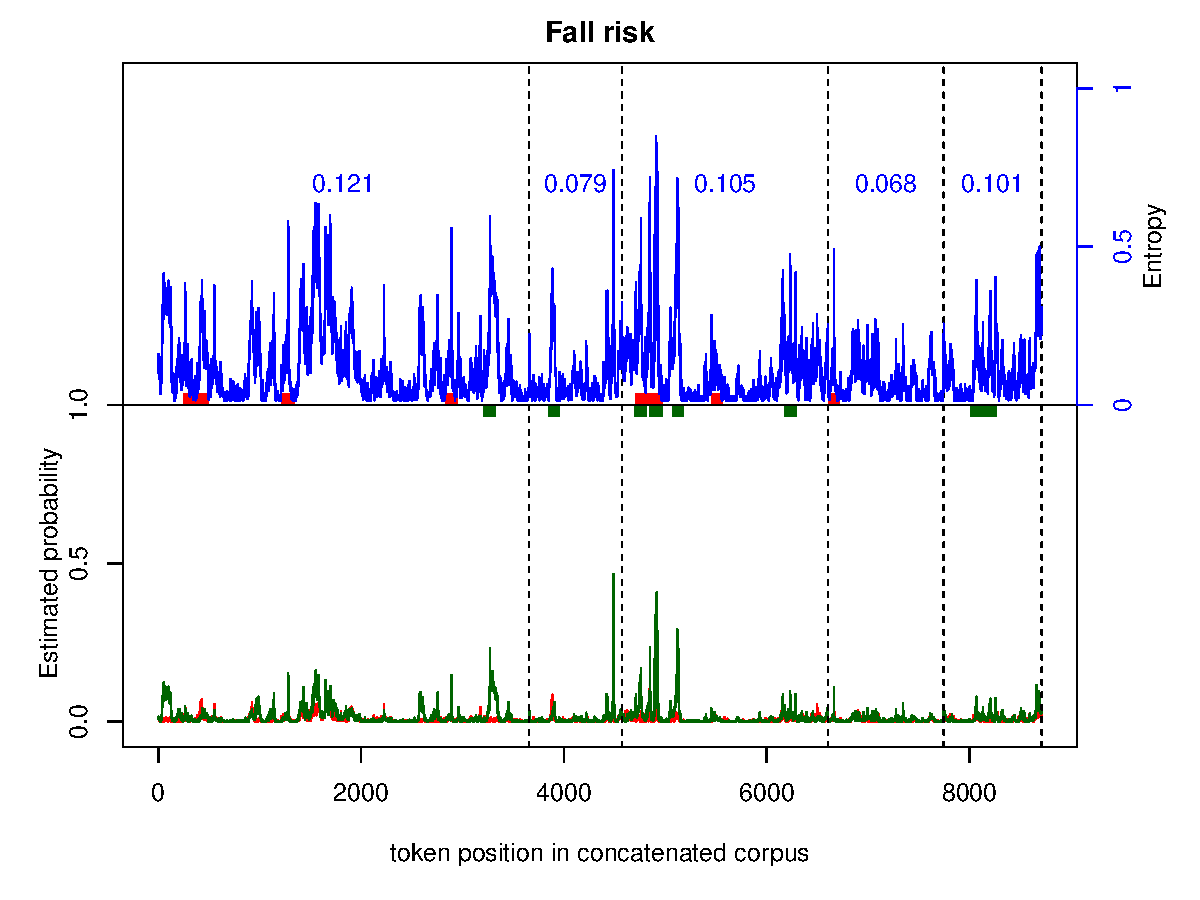
\includegraphics[width = 1.09\textwidth]{/Users/crandrew/projects/GW_PAIR_frailty_classifier/figures/exploratory_Fall_risk.pdf}
\end{frame}

\begin{frame}{Results (preliminary)}
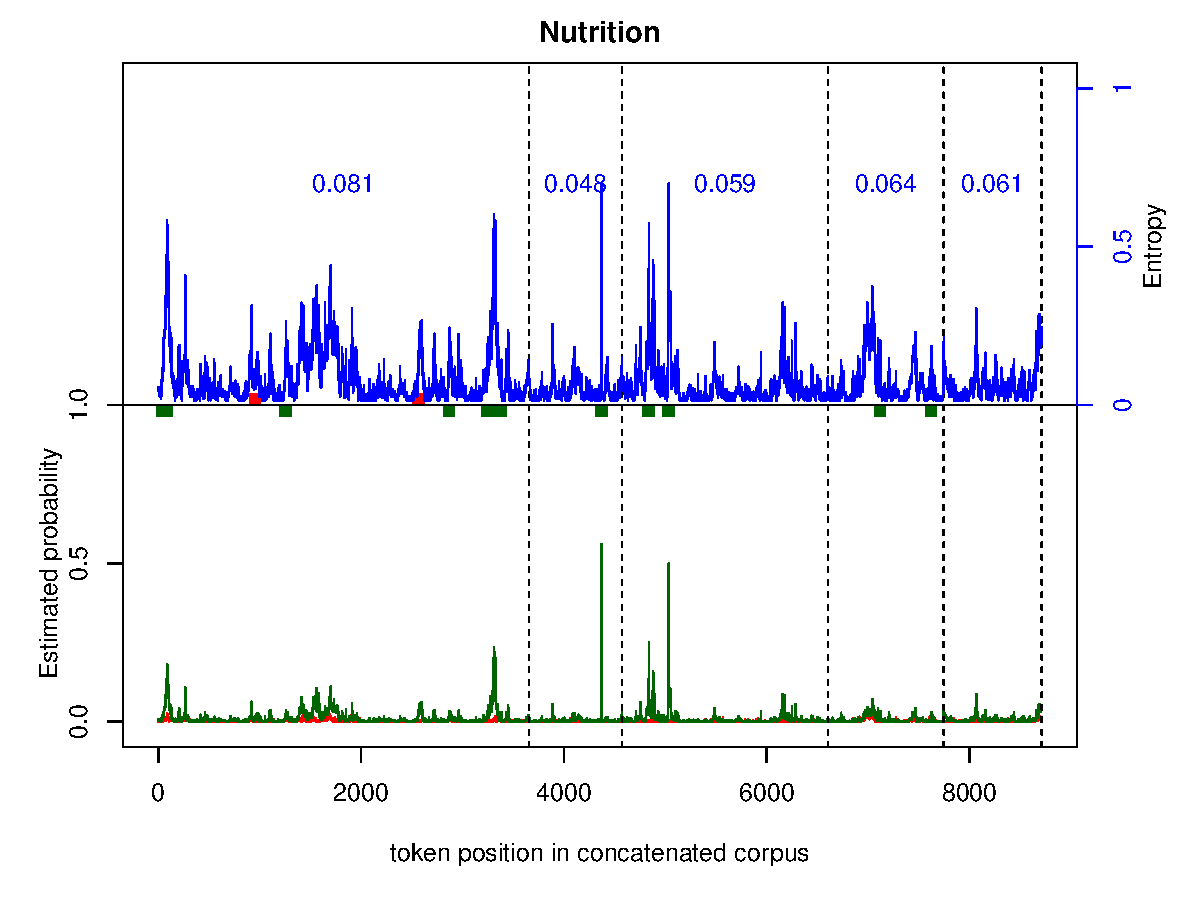
\includegraphics[width = 1.09\textwidth]{/Users/crandrew/projects/GW_PAIR_frailty_classifier/figures/exploratory_Nutrition.pdf}
\end{frame}

\begin{frame}{Results (preliminary)}
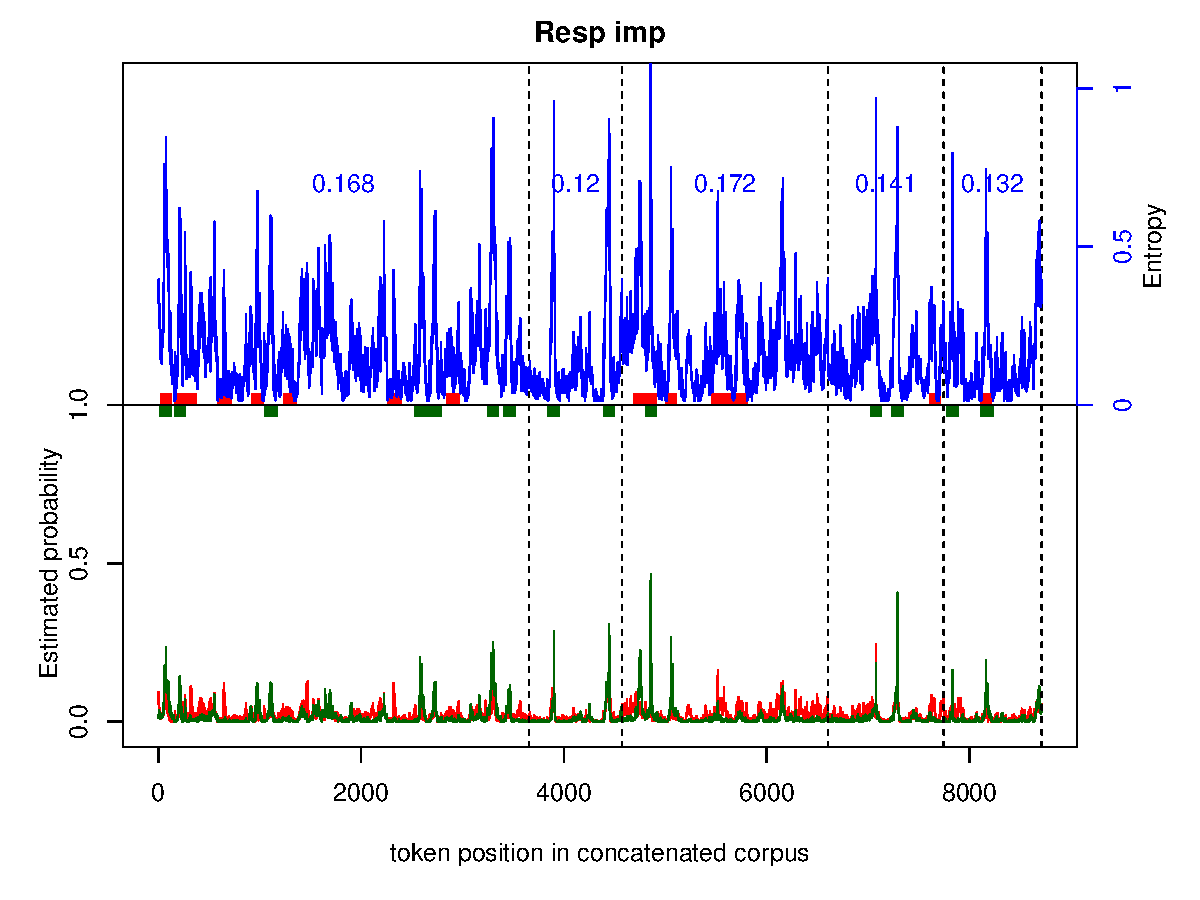
\includegraphics[width = 1.09\textwidth]{/Users/crandrew/projects/GW_PAIR_frailty_classifier/figures/exploratory_Resp_imp.pdf}
\end{frame}

\begin{frame}{Results (preliminary)}
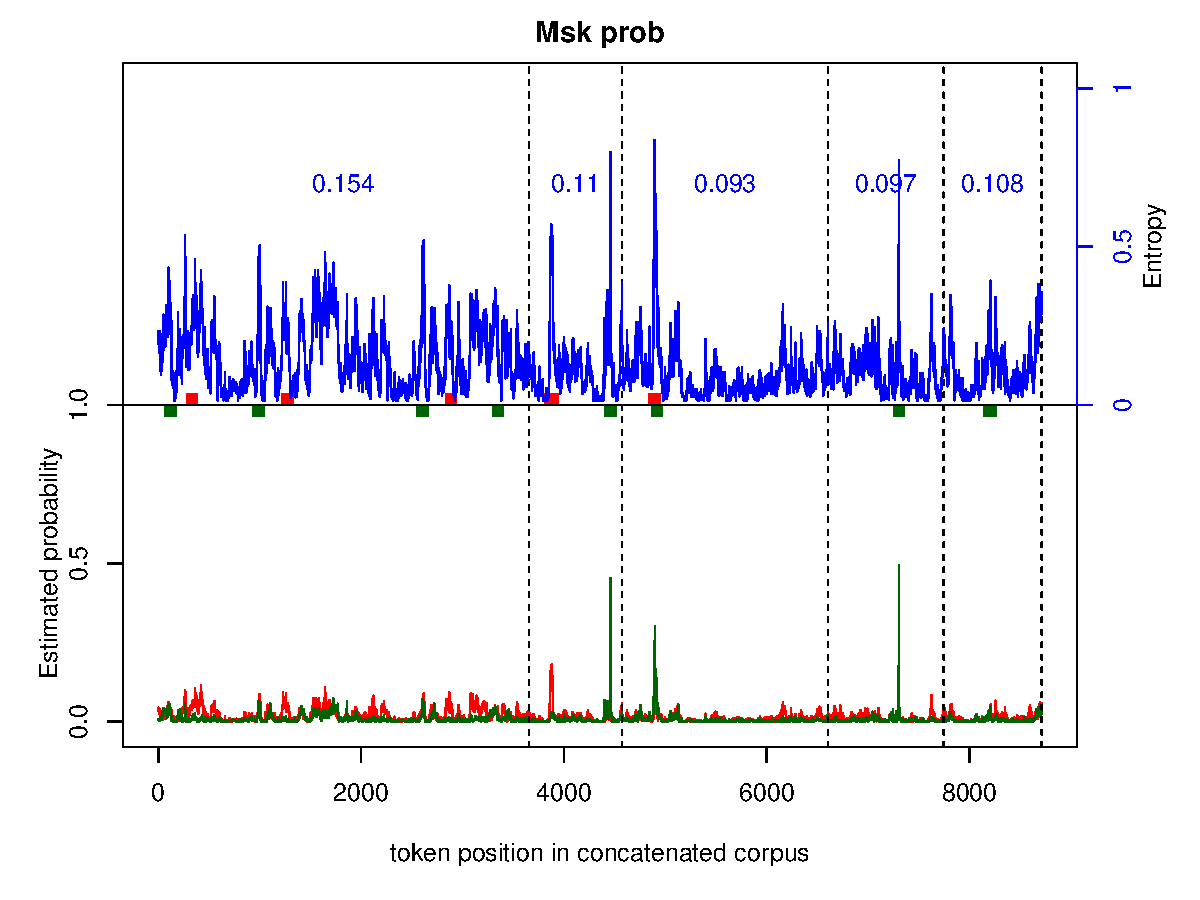
\includegraphics[width = 1.09\textwidth]{/Users/crandrew/projects/GW_PAIR_frailty_classifier/figures/exploratory_Msk_prob.pdf}
\end{frame}


\begin{frame}{Neural nets}
\begin{itemize}
\item I haven't trained a neural net yet
\item I expect that it will be much more efficient
\item Neural nets have the nice feature that they implicitly do the featurization for you
	\begin{itemize}
	\item That's what \textit{representation learning} is, basically
	\end{itemize}
\item That doesn't mean that featurizations fed to the other models wouldn't be useful to the net
	\begin{itemize}
	\item Basically it'd be giving the AI a cribsheet
	\end{itemize}
\item Likewise it'll be important to think carefully about model architecture, especially around questons of context (negation, allusion, etc.)
\end{itemize}
\end{frame}

\begin{frame}{Active learning}
How do we take the output of models fit to the first 25 patient notes and use them to pick the most fruitful notes to annotate next?
\begin{itemize}
\item Standard approach is to pick examples that we're maximally uncertain about
\item \textit{Entropy} is a useful measure of uncertainty from information theory
\end{itemize}
Entropy $\equiv$ H =  $-\displaystyle\sum_{c}p(class = c)log(p(class = c))$
\begin{itemize}
\item It is maximized when you know nothing about which class an example belongs to.
\item We're going to pick notes that have a lot of entropy.
\item Not obvious how best to aggregate entropy over the note.  Thinking perhaps an average over the top quantile.  Maybe decile.
% \item We're going to feed annotators batches of 25 notes at a time.
\end{itemize}
\end{frame}

\begin{frame}{Active learning}
Example:  In the beginning, the model isn't very good and will default to the dominant class (neutral)
\begin{itemize}
\item A token that the model thinks is neutral will have low entropy:  H($[.01, .98, .01] = .11$)
\item If the model thinks that \textit{maybe} another token might be positive, entropy will be a little lower:  H($[.1, .88, .01] = .39$).  That token will make the note more likely to get picked.
\end{itemize}
Eventually, the model will get better about distinguishing the positive classes:
\begin{itemize}
\item After a while, it gets confident about a negative:  E($[.01, .01, .98] = .11$), and that token won't influence what notes get picket to annotate
\item If a note has examples that we are completely uninformed about (maximum entropy), we'd gravitate towards those notes:  H($[.33, .33, .33] = 1.1$)
\end{itemize}
\end{frame}

\begin{frame}{Meta-considerations}
This isn't a causal model, so the usual caveats about feature importance apply
\begin{itemize}
\item That said, it'd be useful to know what sort of features trigger positives and negatives for these frailty aspects
\item Standard permutation importance is usually only done for RF's but can be coded for any model
\end{itemize}
Fairness:
\begin{itemize}
\item What happens if our model is much less certain about patients who are/aren't black/white/men/women/rich/indigent?
\item Do we think it's likely that clinicians write differently about patients who are different -- consciously or unconsciously, intentionally or otherwise?
\item Can we apply post-hoc statistical fixes to correct for such biases?
\end{itemize}
\end{frame}

\begin{frame}{Wrapup}
Takeaways, challenges, and points to discuss:
\begin{itemize}
\item We are annotating and predicting labels on spans of text, but
	\begin{itemize}
	\item how do we classify actual patients?
	\end{itemize}		
\item Context is critical in text modeling.  
	\begin{itemize}
	\item What are the best ways to represent it?
	\end{itemize}		
\item After the first batches of notes, we're going to pick subsequent notes about which we're maximally uncertain.  
	\begin{itemize}
	\item But what is the best way to aggregate that uncertainty?
	\end{itemize}		
\item Bias is likely to pop up along the way.  
	\begin{itemize}
	\item How can we plan for it?
	\end{itemize}		

\end{itemize}
\end{frame}

\begin{frame}
\huge{\textbf{Thanks!}}
\end{frame}


\end{document}